% This version uses the latex2e styles, not the very ancient 2.09 stuff.
\documentclass{sig-alternate-10pt}
\usepackage{endnotes,url}
%\usepackage{sig-alternate-10pt,endnotes}
\usepackage{epsfig}
\usepackage{amssymb}
\usepackage{amsmath}
\usepackage{lipsum}
\usepackage{algorithm}
\usepackage{algorithmic}
\usepackage{amsfonts}
\usepackage{graphicx}
\usepackage{verbatim}
% Replaced by subfig package
% \usepackage{subfigure}
\usepackage{subfig}
\usepackage{epstopdf}
\usepackage{cite}
\usepackage{array}
\usepackage{multirow}
\usepackage{listings}


\captionsetup[figure]{labelfont={small},textfont={small}}

%\pdfpagewidth 8.5in
%\pdfpageheight 11in
%\baselineskip=12.5pt
%\setlength{\pdfpagewidth}{8.5in}
%\setlength{\pdfpageheight}{11in}
%\usepackage{pdfdraftcopy}

% To import classical math notation used

% Mathematical LaTeX formatting shortcuts
\newcommand{\midwor}[1]{\;\textnormal{ #1 }\;} % text in math mode
\newcommand{\ds}{\displaystyle} % shorcut to toggle display
	% All formula should punctuation as they are part of the text.
\newcommand{\vf}{\,,\,} % a comma with space
\newcommand{\ff}{\,.} % a dot 
	% The following command allows to write quickly sets { }   
\newcommand{\lset}{\left\{\left.\;}
\newcommand{\midset}{\;\right|\;\left.}
\newcommand{\dimset}{\right.\;\left|\;}
\newcommand{\rset}{\;\right.\right\}}
\newcommand{\jset}{\right.\right.\\ & \left.\left.}

% Number sets and usual operations
\newcommand{\Real}{\mathbb{R}} % real numbers
\newcommand{\RelInt}{\mathbb{Z}} % relative integer numbers
\newcommand{\NatInt}{\mathbb{N}} % natural integer numbers
\newcommand{\Compl}{\mathbb{C}} % complex numbers
\newcommand{\valent}[1]{\left\lfloor #1 \right\rfloor} % integer value
\newcommand{\valentsup}[1]{\left\lceil #1 \right\rceil} % integer value + 1
\newcommand{\eps}{\varepsilon} % very small real number
\newcommand{\argmin}{\textrm{argmin}} %argument of the minimum
\newcommand{\pospar}[1]{\left( #1 \right)^+} % positive part

% Probability notation
\newcommand{\proba}{\mathbb{P}} % Probability
\newcommand{\probaof}[1]{\mathbb{P}\left.\left[#1\right.\right]} % Probability of an event
\newcommand{\cond}{\right|\left.} % Condition on an event 
\newcommand{\expec}[1]{\mathbb{E}\left[#1\right]} % Expectation 
\newcommand{\vari}[1]{\textrm{V}\left[#1\right]} % Variance 
\newcommand{\Lun}{\mathbb{L}^{1}} % Space of integrable function
\newcommand{\as}{\;\textrm{a.s.}\;}
\newcommand{\ind}[1]{\mathbb{I}_{\{#1\}}} % Indicator
\newcommand{\tribF}{\mathcal{F}} % sigma-algebra

% Constants
\newcommand{\cst}{\textrm{\texttt{cst}}}

% Advanced probability 
\newcommand{\comp}{\circ} % composition of function
\newcommand{\shi}{\theta} % ergodic shift
\newcommand{\lstoc}{\displaystyle \leq_{\textrm{st}}} % Stochastic Order
\newcommand{\Ppalmof}[1]{\mathbb{P}^{0}_{#1}}
\newcommand{\Pofpalmof}[2]{\mathbb{P}^{0}_{#1}\left[#2\right]}
\newcommand{\expPalm}[1]{\mathbb{E}^{0}[#1]} % Palm Expectation
\newcommand{\expPalmof}[2]{\mathbb{E}^{0}_{#1}[#2]} % Palm Expectation w.r.t. point process f 

% (max,+) algebra
\newcommand{\Rmax}{\mathbb{R}_{\max}}
\newcommand{\ninf}{\varepsilon}
\newcommand{\matninf}{\textrm{\Large{$\ninf$}}}
\newcommand{\zer}{e}
\newcommand{\veczer}{\textrm{\Large{e}}}
\newcommand{\bigmax}{\bigvee}
\newcommand{\matId}{{\mathbb{I}}}
%\newcommand{\norm}[1]{\| #1 \|}
\newcommand{\linf}[1]{\left|\left| #1 \right|\right|}

% Matrices
\newcommand{\matA}{\mathbb{A}}
\newcommand{\matB}{\mathbb{B}}
\newcommand{\matC}{\mathbb{C}}
\newcommand{\matP}{\mathbb{P}}
\newcommand{\matQ}{\mathbb{Q}}

% Used for set
\newcommand{\setI}{\mathcal{I}}
\newcommand{\setJ}{\mathcal{J}}
\newcommand{\setK}{\mathcal{K}}
\newcommand{\setL}{\mathcal{L}}

% Users and Buckets
\newcommand{\setU}{\mathcal{U}}
\newcommand{\setC}{\mathcal{C}}

\newcommand{\setA}{\mathcal{A}}
\newcommand{\setW}{\mathcal{W}}

% Used for set
\newcommand{\setN}{\mathcal{N}}
\newcommand{\setS}{\mathcal{S}}


\newenvironment{disarray}%
 {\everymath{\displaystyle\everymath{}}\array}%
 {\endarray}

 \newcommand{\pdi}[1]{\frac{\partial #1}{\partial x_i}}
 \newcommand{\pdj}[1]{\frac{\partial #1}{\partial x_j}}

% Package for date and time presentation
\usepackage{datetime}
\newcommand{\datation}{\today, \xxivtime}

\def\full{0}        % set 1 for a full tech report version
                    % set 0 for submission version
\def\shownotes{1}   % set 1 for version with author notes
                    % set 0 for no notes
\def\anon{1}        % set 1 to anonymize
                    % set 0 for acks and author names

%%%%%%%  Author Notes %%%%%%%
%
\ifnum\shownotes=1
\newcommand{\authnote}[2]{{ $\ll$\textsf{\footnotesize #1 notes: #2}$\gg$}}
\else
\newcommand{\authnote}[2]{}
\fi
\newcommand{\Anote}[1]{{\authnote{Andrius}{#1}}}

%%%%%%%%%%%%%%%%%%%%%%%%%%%%%%%%%

\newcommand{\namedref}[2]{#1~\ref{#2}}
\newcommand{\tableref}[1]{\namedref{Table}{#1}}
\newcommand{\sectionref}[1]{\namedref{Section}{#1}}
\newcommand{\appendixref}[1]{\namedref{Appendix}{#1}}
\newcommand{\theoremref}[1]{\namedref{Theorem}{#1}}
\newcommand{\remarkref}[1]{\namedref{Remark}{#1}}
\newcommand{\definitionref}[1]{\namedref{Definition}{#1}}
\newcommand{\figureref}[1]{\namedref{Figure}{#1}}
\newcommand{\lemmaref}[1]{\namedref{Lemma}{#1}}
\newcommand{\claimref}[1]{\namedref{Claim}{#1}}
\newcommand{\propositionref}[1]{\namedref{Proposition}{#1}}
\newcommand{\constructionref}[1]{\namedref{Construction}{#1}}
\newcommand{\corollaryref}[1]{\namedref{Corollary}{#1}}
\newcommand{\equationref}[1]{\namedref{Equation}{#1}}
%
\newtheorem{theorem}{Theorem}[section]
\newtheorem{definition}[theorem]{Definition}
\newtheorem{lemma}[theorem]{Lemma}
\newtheorem{claim}[theorem]{Claim}
\newtheorem{obs}[theorem]{Observation}
%


\providecommand{\vs}{vs. }
\providecommand{\ie}{\emph{i.e.,} }
\providecommand{\eg}{\emph{e.g.,} }
\providecommand{\cf}{\emph{cf.,} }
\providecommand{\resp}{\emph{resp.,} }
\providecommand{\etal}{\emph{et al.}}   %Removed trailing space here; usually want non-breaking space with following reference
\providecommand{\etc}{\emph{etc.}}      % No trailing space here either
\providecommand{\mypara}[1]{\smallskip\noindent\emph{#1} }
\providecommand{\myparab}[1]{\smallskip\noindent\textbf{#1} }
\providecommand{\myparasc}[1]{\smallskip\noindent\textsc{#1} }
\providecommand{\para}{\smallskip\noindent}

\newtheorem{axiom}{{\bf  Axiom}}
\newtheorem{defin}{{\bf  Definition}}
\newtheorem{proposition}{Proposition}

\usepackage{enumitem}
\setlist{nolistsep}

%Model parameters

\usepackage[breaklinks=true]{hyperref}
\frenchspacing
\begin{document}

%don't want date printed
\date{}


%make title bold and 14 pt font (Latex default is non-bold, 16 pt)
\title{NoTCP: steganographic tricks to bypass middleboxes}
\ifnum\anon=1
\author{[Paper: \#137]}% \hspace{0.2cm} \ampmtime ]}
\else
\numberofauthors{3}
\author{
\alignauthor Andrius Aucinas\\
\affaddr{University of Cambridge} 
\and
\alignauthor Jon Crowcroft\\
\affaddr{University of Cambridge}
\and
\alignauthor Narseo Vallina-Rodriguez\\
\affaddr{ICSI}
}
\fi
%for single author (just remove % characters)

    
% end author
\maketitle
% Use the following at camera-ready time to suppress page numbers.
% Comment it out when you first submit the paper for review.
%\thispagestyle{empty}
\begin{abstract}
TCP is the de facto transport protocol in the Internet. However it has many limitations that make it ill suited to the modern world of high mobility and multi-homing. Protocol optimizations and filtering performed by middleboxes make extension deployment challenging which has led researchers to explore new ways of exchanging control information between endpoints. In this paper we explore steganographic approaches to smuggle information between endpoints. We design NoTCP -- a mechanism which uses the TCP header fields in combinations that are currently have no defined semantics to hide a small amount of control information from middleboxes and hence bootstrap a control channel. We also present a preliminary study showing how the mechanism works across cellular and WiFi networks.
\end{abstract} 

\section{Introduction}
\label{section:intro}

TCP is everywhere in the Internet. The overwhelming majority of bytes are carried in TCP streams~\cite{John:2007dv}, and TCP is used for all types of traffic from bulk download to video streaming to instant messaging. Over the last decade a number of new protocols have been proposed to replace TCP. However many middle boxes will actively block or interfere with traffic that does not conform to their view of what TCP should look like. Consequently few of these protocols have found any leverage.

One of the main requirements to extend and modify TCP is the ability to exchange control information. Traditionally this is what TCP option space was used for. However option space is limited, heavily contended~\cite{Handley:vj,Mazieres:uz} and troubled by network middleboxes~\cite{Honda,Guha2005tb,UntoldMiddlebox2011}.

Instead we believe that the solution is to work round the middle boxes by using steganographic techniques~\cite{Frczek:2012dl,Zielinska:2014fn,Rowland:1997vq,Murdoch:2005fz} to conceal control information within the TCP header. This could be as simple as using one of the currently undefined flags to toggle the meaning of existing fields, through to using the urgent pointer without setting the urgent flag or even hashing information into the initial sequence number in much the way that SYN Cookies~\cite{Eddy:2007to} do currently.

A practical method of exchanging control information outside of TCP options could not only speed up deployment of existing TCP extensions (\eg MPTCP~\cite{Handley:vj}, TCPCrypt~\cite{Mazieres:uz}), but also help add a generic control stream within TCP. Potential applications range from new secure extensions~\cite{Rescorla:R080FoGB} to exchanging information about endpoints for connection parameter tuning (\eg initial congestion window~\cite{Dukkipati:2010hs}) to designing better coordination for long-lived connections to save mobile device energy~\cite{Aucinas:2013uk}. Most importantly, development of new functionality should not be limited by network middleboxes.

This paper makes three main contributions. 
\begin{enumerate}
\item We discuss the possible ways to conceal information in the TCP header and give some examples of the extensions this could enable
\item We describe a measurement application that we have written to run on Android phones.  
\item We present the results of a small scale deployment of our application.
\end{enumerate}

Our hope is to motivate the research community into exploring the full range of possibilities in this space and to encourage more people to install our application so that we can build a comprehensive database of the impact of middleboxes across different network providers.

% Extensibility of the Internet has been not like originally envisioned for a long time now, starting with IP layer and extending the \emph{narrow waist} to TCP or even HTTP at large. The problem is caused by the various middleboxes that aim to improve performance\cite{Kopparty:2002ht,Chakravorty:2003dm}, increase security\cite{Handley:2001vp,Vutukuru:2008fc} and solve address shortage problems. Even congestion control has required multiple extensions since protocol's inception and the large number of proposed congestion control schemes~\cite{5462976} suggests that more will be necessary.

% In an ideal world all infrastructure is forwards compatible and changes together with the needs of the users. Instead, TCP has become the de facto transport protocol of the Internet and development of its extensions has been very challenging. Proposals including MPTCP~\cite{Handley:vj} for multi-homed endpoints and TCPCrypt~\cite{Mazieres:uz} for ubiquitous end-to-end traffic encryption are necessary for today's networks but deployment has been slow and difficult. Previous work on MPTCP overviews the major problems with different types of middleboxes~\cite{Raiciu:2012ur}.

% Although TCP has been built to be extensible via options and reserved bits, all extensions are primarily designed around the limitations of existing network middleboxes\cite{Honda,Guha2005tb,UntoldMiddlebox2011}, but even if options were not filtered, we have run out of the 40-byte TCP option space.

% Problems with the size of option space arise in MPTCP when its options are combined with those of regular TCP and therefore needs to change the semantics of a duplicate ACK~\cite{Handley:vj} and there are efforts to define an alternative control stream to work around the limitation of option space~\cite{Bonaventure:wx}. TCPCrypt uses the Data portion of TCP segments to exchange cryptographic keys~\cite{Mazieres:uz}. An alternative way of looking at the problem is to hide the information from the middleboxes as done by steganographic approaches~\cite{Frczek:2012dl,Zielinska:2014fn,Rowland:1997vq,Murdoch:2005fz}.

% We propose \emph{noTCP}, an approach complementary to option negotiation which repurposes TCP header fields beyond what is specified. At the same time it is designed to work across most of deployed network infrastructure. At the core of the idea is modification of TCP header fields in a way that is not interfered with by middleboxes or so that such interference can be safely recovered or ignored. The idea builds up from the work on steganography using TCP~\cite{Frczek:2012dl,Murdoch:2005fz}, but we shift the focus from using sequence numbers and options to other fields as well.

% With the focus on cellular and WiFi networks due to their renown middlebox peculiarities, we make the following contributions in this work:

% \begin{enumerate}
%     \item Review the aspects of the TCP protocol that can potentially be used to extend it (Section~\ref{sec:protocolChanges}).
%     \item Provide an analysis of current mobile (WiFi and cellular) network behavior in the presence of such modifications (Section~\ref{sec:network}).
%     \item Propose a robust method to bootstrap control-stream between two endpoints across middleboxes (Section~\ref{sec:protocol}).
% \end{enumerate}

\section{Candidate protocol changes}
\label{sec:protocolChanges}

\begin{figure}[t!]
\centering
\small{
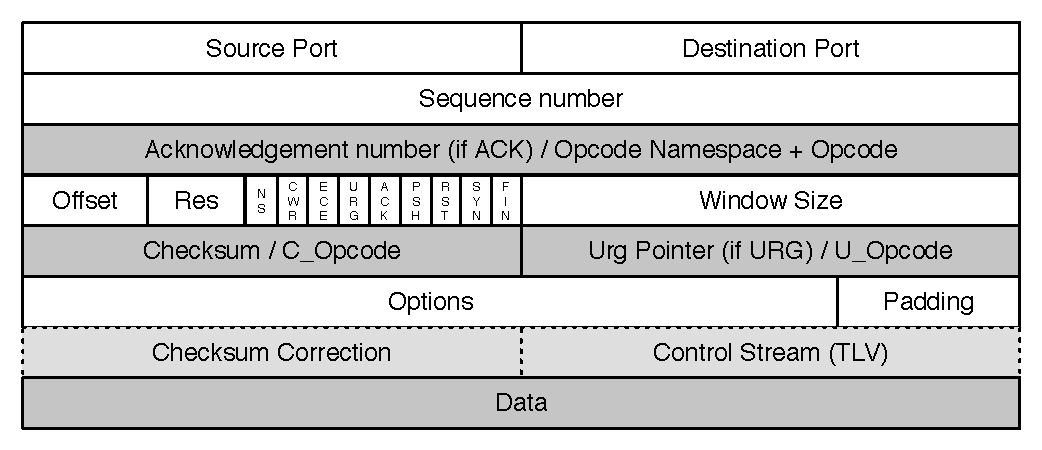
\includegraphics[width=\columnwidth]{figs/tcp-header}
\vspace{-3mm}
\caption{TCP Header with overloaded fields and extra control information (Checksum Correction / Control Stream) in payload}
\label{fig:header}
}
\vspace{-2mm}
\end{figure}

Without using the options field we only have a few options for control information exchange:
\begin{itemize}
    \item Setting header fields to specific values without setting the corresponding flags to have no meaning to legacy implementations.
    \item Assigning one or more of the reserved field bits.
    \item Defining new semantics for valid header fields.
\end{itemize}

In this section we discuss them and their pros and cons in depth. Fig.~\ref{fig:header} shows TCP header with fields that we propose for reuse and define in Section~\ref{sec:protocol}.

\subsubsection*{Unset Flags}
\label{sec:unset}

The only header fields that may not have a meaning depending on the corresponding flag are \emph{Urgent Pointer} and \emph{Acknowledgment Number}. The latter must always be set after the initial SYN packet.

It is recommended against the use of the urgent mechanism~\cite{Gont:2011vi}, therefore it could be reused for other purposes if both endpoints understand the new semantics. On the other hand, it is common practice by Network Intrusion Detection Systems (NIDS) on enterprise networks to reset the field as it makes it difficult to track application-layer data~\cite{seolma}. Better yet, the field becomes \emph{Non-Urgent}~\cite{Kuhlewind:2014vd} when URG is not set -- it has no meaning for legacy implementations and can be redefined.

Acknowledgment field is only available in the initial SYN packet. It must therefore be combined with another mechanism to acknowledge control information unless TCP Simultaneous Open is used. Simultaneous open is still viable in most cellular networks~\cite{UntoldMiddlebox2011}, but we also explore other options.

\subsubsection*{Reserved bits}

Only 3 TCP Reserved bis have been left unallocated with the three ECN bits (ECN, CWR and experimental NS)~\cite{Floyd:up,Ely:uc} that are still not universally implemented~\cite{Kuhlewind:2013hr}.

Due to simplicity and non-interference with legacy implementations there are proposals that make use of them. One suggestion for reducing Web latency~\cite{Flach:2013uy} by mitigating the effects of a small number of lost packets for short connections is to send multiple copies of packets. To avoid triggering duplicate acknowledgments reserved bit is used to mark such packets as duplicate and should be ignored by fast retransmit.

\subsubsection*{Value-specific semantics}

The remaining choice is to encode information within valid header fields. It involves generating packets with specific values for initial sequence numbers, window size or checksums. We posit that it would be an acceptable choice as long as it is deployable in today's network.

Initial sequence numbers must be hard to predict as they provide a measure (however weak) of security and until strong encryption, \eg TCPCrypt, is universally adopted. Adding any information to the field in a way that is easily decoded by the receiver makes it predictable and weakens security  which has already been problematic~\cite{Qian:2012bj,Bellovin:uz,Qian:2012wb}. 

Window size is potentially a better candidate, especially if used during connection setup phase since data is not typically transmitted during the handshake. Using lower-order bits for control information would prevent flow control from operating properly, but higher-order bits could instead be given up when window scaling option is used to compensate for the decrease of advertised window size. Using the field risks interfering both with TCP flow control mechanism as well as window size optimizations by the network~\cite{Kopparty:2002ht,Chakravorty:2003dm} performed \eg by Citrix ByteMobile Proxy~\cite{Ha:2006td}. 

There are multiple benefits to using the checksum field. Firstly, it is only used for error detection. It may be unnecessary when reliable error detection is done at the layer below, however link-level checks have been shown unreliable~\cite{Stone:2000fc}. Instead, it may be replaced with extensions' separate, potentially stronger mechanisms \eg MPTCP DSS checksum and TCPCrypt Message Authentication Code) or left for the upper layer.

Secondly, checksum operations are efficient as they only involve one's complement addition. We show later in the paper (Section~\ref{sec:protocol}) how checksums can be generated in a way that the intended value is recovered by the receiver after traversing multiple layers of Network Address Translation (NAT).

\section{Methodology}

To verify current network behavior we have developed an Android application distributed through the \emph{Google Play Store} to collect data from volunteers. It contains a simplified implementation of TCP to generate packet sequences that appear valid to network middleboxes: three-way handshake, data exchange and connection teardown. It allows us to modify various header fields to our purposes and check the values received by the other endpoint.

The testing setup is:
\begin{itemize}
    \item Android UI to launch tests, report aggregated results to the end-users, send results to the reporting server and manage the tests.
    \item Simplified TCP stack using Raw Unix sockets for full control over the TCP header (\emph{SOCK\_RAW}). %This also meant having to drop RST packets generated by the kernel network stack during the test in response to incoming packets associated with connections it is not aware of - packets are delivered to both the raw socket and the kernel network stack.
    \item Server instrumented to generate specific responses to incoming packets based on header and payload values. We currently use a dedicated test server in a single location and no firewalls or NATs.
\end{itemize}

Non-transparent proxies are a major problem for extension deployment, therefore we used another well know and widely deployed tool to detect proxies on our tested networks. The tests were run separately, using previously developed techniques~\cite{Weaver:RHwbx82O}. The primary one was non-responsive server test: the server is instrumented not to respond to SYN, therefore if connection succeeds it is to a proxy on the path. We repeated these tests on different destination ports and found that proxying can be specific to certain port numbers (Section~\ref{sec:portspec})

Transparency of proxies may also depend on higher-level protocols, therefore we checked for HTTP proxies using techniques proposed in the work, including checking content and header changes, different IP addresses seen for HTTP or non-HTTP traffic, whether non-HTTP traffic on HTTP port is filtered, HTTP traffic is normalized (\ie deliberately modified headers are fixed). We control both endpoints of each connection, therefore we can detect changes from sent values received by the other endpoint. Results are presented in Section~\ref{sec:proxies}.

\subsection{Limitations}

Potential limitations of our methodology include that we do not consider packet splitting and coalescing. Our goal is to exchange control information within packet headers that correct behavior does not depend on how packets are resegmented. To ensure that it does not happen during our tests we do not send more than a few bytes of data and the exchange only consists of a single message sent each way. Due to the same reason we do not take congestion control into account either.

Raw sockets operate in parallel to the kernel network stack. We had to suppress reset packets generated by the kernel in response to TCP packets from sessions it is not aware of. We also had to choose local port numbers unused by the kernel. We chose them randomly from the unprivileged port range and relied on other error detection mechanisms to prevent invalid packets from being delivered in the unlikely case of coinciding connection parameters. 

\section{Network characteristics}
\label{sec:network}

\begin{table*}[t]
{\small
\begin{center}
\begin{tabular}{| l | >{\centering\arraybackslash}m{1.2cm} | >{\centering\arraybackslash}m{1.6cm} | >{\centering\arraybackslash}m{1.6cm} | >{\centering\arraybackslash}m{1.8cm} | >{\centering\arraybackslash}m{1.6cm} | >{\centering\arraybackslash}m{1.5cm} | >{\centering\arraybackslash}m{1.5cm} | >{\centering\arraybackslash}m{1.5cm} | >{\centering\arraybackslash}m{1.cm} | }
\hline
    \textbf{Net ID} & \textbf{Country} & \textbf{Port-specific} & \textbf{Validate checksum} & \textbf{Drop SYN-ACK data} & \textbf{Normalize SYN Ack number}  & \textbf{Normalize Urgent Pointer} & \textbf{Normalize Reserved} & \textbf{Remap Sequence} \\ \hline \hline
    % Univ Helsinki WiFi
    WiFi edu 1      & Finland               &                        & \checkmark                 &                        &                         &                        &                             &                     \\ \hline
    % Eduroam
    WiFi edu 2      & UK               &                        &                            & \checkmark             &                         & \checkmark             &                             & \checkmark          \\ \hline
    % wgb
    WiFi pub 1      & UK               &                        &                            &                        &                         &                        &                             &                     \\ \hline
    % MKSW germany (carlos)
    WiFi pub 2      & Germany               &                        & \checkmark                 & \checkmark             &                         &                        &                             &                     \\ \hline
    % Virgin home
    WiFi res 1      & UK               &                        & \checkmark                 &                        &                         &                        &                             &                     \\ \hline
    % TEO Lt
    WiFi res 2      & Lithuania               &                        & \checkmark                 & \checkmark             &                         &                        &                             &                     \\ \hline
    % Telefonica Free
    WiFi ent 1      & Spain               &                        & \checkmark                 & \checkmark             &                         &                        &                             &                     \\ \hline
    \hline
    % Finland internet.saunalahti
    Cellular 1      & Finland               &                        &                            &                        &                         &                        &                             &                     \\ \hline
    % GiffGaff
    Cellular 2      & UK               &  443, 993              & -                          & -                      & -                       & -                      & -                           & -                   \\ \hline
    % E-Plus germany
    Cellular 3      & Germany               &                        &                            &                        &                         & \checkmark             &                             & \checkmark          \\ \hline
    % EE/T-Mobile
    Cellular 4      & UK               &               80, 443  & -                          & -                      & -                       & -                      & -                           & -                   \\ \hline
    % Three UK
    Cellular 5      & UK               &                        & \checkmark                 &                        &                         &                        &                             &                     \\ \hline
    % Omnitel LT
    Cellular 6      & Lithuania               &                        & \checkmark                 &                        &                         &                        &                             &                     \\ \hline
\end{tabular}
\end{center}
}
\caption{Network behavior observed through tests generating custom TCP packets. A dash means different cases observed based on port numbers.}
\label{tab:networks}
\end{table*}

We show our collected results in Table~\ref{tab:networks}. Since we were focusing on mobile applications, in our preliminary study we collected results across a few public, residential, university and enterprise WiFi networks as well as 6 cellular networks in 4 different countries: UK, Finland, Germany and Lithuania.

The results include which networks did not filter any modifications (one WiFi and two cellular nets), and which ones discarded packets with invalid checksums, normalized particular fields - either dropped packets or reset to different values - and whether NATs performed only port number remapping or also changed sequence numbers. Only one network provided clients with a global IP (WiFi edu 2).

In traditional NATs~\cite{Egevang:tu} checksum recalculation is very simple: subtract the old header fields from the checksum and add the new ones to minimize the resource use. The networks that deliver packets with invalid checksum only do that as otherwise a packet with invalid checksum would be dropped.

A bigger issue we have discovered is that middleboxes do not always respect the standard and simply drop SYN-ACK packets with payload. We did not see it on cellular networks, but most WiFi (4/7) behaved in such way even though the standard allows handshake packets to contain payload~\cite{Postel:3EDyoxP_,Chu:2011tn}.

% \begin{quotation}
%     Although these examples do not show connection synchronization using data-carrying segments, this is perfectly legitimate
% \end{quotation}

As discussed in Section~\ref{sec:unset}, we can squeeze in a few extra bits of information by defining meaning to header fields when corresponding flags are not set. None of our tested networks filtered Acknowledgment Number field for the initial SYN packet on non-proxied paths and only two networks discarded packets with Urgent Pointer set without URG flag.

Finally we tested interaction reserved header bits. We separated our tests to handshake and data exchange parts as well as set each bit individually, however we did not observe different behavior for these: all reserved bits were either allowed through or cleared at both phases. Importantly, we did not observe cases when such packets are dropped.


\subsection{Port-specific middlebox behavior}
\label{sec:portspec}

We repeat our tests on a few ports:
\begin{itemize}
    \item 80, 443 - HTTP and HTTPS
    \item 993 - Secure IMAP port
    \item 5228 - Google cloud messaging port
    \item 6969 - random port number
    \item 8000 - common HTTP proxy port number
\end{itemize}

We only observed port-specific behavior on two networks: \emph{Cellular 2} and \emph{Cellular 4}. In the first case, traffic travels over SSL ports (443, 993) unmodified except for packets with invalid checksum being dropped. Our traffic was not encrypted and an increasing proportion of traffic is served over SSL. A commercially deployed HTTP accelerator reports the proportion of HTTPS requests to be close to that of HTTP\footnote{\url{http://db.awazza.com/users/global/}}, making the value of such proxying questionable.

We confirmed the middlebox to be a ByteMobile proxy. It replaces the original connections with a new one which adds options not present in original packets, changes window size and resets other fields to new values to optimize TCP for cellular networks~\cite{Ha:2006td}. Such behavior makes deployment of any protocol modifications or extensions very difficult (e.g. we verified that TCPCrypt does not work on this network). Although we did not see more cases of it, the company claims over 160 clients.

In the second case, traffic was only modified when going to ports 80 and 443. As we discuss below, the network optimizes HTTP traffic and since our traffic does not resemble valid HTTP, it is dropped.

\subsection{Non-transparent proxies}
\label{sec:proxies}

Since proxies make new changes very difficult, we checked for non-transparent oes on in our tested networks on a number of popular port numbers:
21, 22, 25, 80, 110, 135, 139, 143, 161, 443, 445, 465, 585, 587, 993, 995, 1194, 1723, 5060, 6881, 9001.

\begin{table}[t!]
{\small
\begin{center}
\begin{tabular}{| l | >{\centering\arraybackslash}m{1.8cm} | >{\centering\arraybackslash}m{3.7cm} |}
\hline
    \textbf{Net ID} & \textbf{Radio Technology} & \textbf{Proxied Ports} \\ \hline \hline
    Cellular 2      & HSPA                      & 21, 22, 25, 80, 110, 135, 143, 161, 465, 585, 587, 995, 1194, 1723, 5060, 6881, 9001 \\ \hline
    Cellular 4      & GPRS                      & 80, 110, 143 \\ \hline
    Cellular 4      & HSPA                      & 80, 110, 143 \\ \hline
    Cellular 4      & LTE                       & 80, 110, 143, 443, 993, 995 \\ \hline
    % T-Mobile, part of EE
    Cellular 4*     & HSPA                     & 25, 80, 110, 143 \\ \hline
    % Virgin on T-Mobile
    Cellular 4**    & HSPA                    & 25, 80, 110, 143 \\ \hline
\end{tabular}
\end{center}
}
\vspace{-2mm}
\caption{Non-transparent proxies and proxied port numbers by radio technology}
\label{tab:proxies}
\vspace{-4mm}
\end{table}

Results are summarized in Table~\ref{tab:proxies}. Cellular 2 proxies almost all of our tested ports except for 443 and 993 as observed before. 
Cellular 4 shows non-uniform behavior across the network. It is not obvious why ports commonly used for encrypted communication are proxied over LTE, we only recorded 1 case for HTTPS. The other two cases (* and **) seem related to the operator being formed from two merged operators. These differences are evident in \emph{whois} records and device-reported network name --- \textbf{*} shows the old operator name and \textbf{**} reports the name of a virtual network operator (MVNO), which rent network infrastructure from the mobile network operator.

It is not safe to estimate proxying just from \emph{whois} records: they do not necessarily match the operator names and we saw the same address ranges used with all device-reported network names for HSPA and LTE radios. An active test is needed reliably detect proxies.

Proxying is protocol-dependent in some cases: looking at port 80, Cellular 4\*\* modified HTTP headers, performed transcoding and reordered header fields, but only modified non-HTTP traffic for one of the two sessions. While other networks did not interfere with our tests, they do not appear to be completely free of proxies. On Cellular 1 (15 sessions) two sessions show DNS proxies and on Cellular 5 two sessions (out of 47) had non-HTTP traffic filtered on port 80. Finally, Cellular 2 and 4 both reorder HTTP headers and perform transcoding, but Cellular 4 does not always allow non-HTTP traffic. We did not have data about Cellular 6, but results discussed above suggest that there are no non-transparent proxies present.

All other networks did not show non-transparent proxy behavior, but the ones who did pose a challenge that is not easily solved. Proxies potentially change every aspect of the original connection and hiding any information within the packet becomes extremely difficult since any value that a proxy does not recognize is reset.


%    an_op_name    | an_cell_net_type | an_country | port |    ip_global (simplified to network address. Included the owner according to whois
% db)
% -----------------+------------------+------------+------+-----------------
%  EE              | GPRS             | gb         |   80 | 31.72/19 (EE)
%  EE              | GPRS             | gb         |  110 | 31.72/19 (EE)
%  EE              | GPRS             | gb         |  143 | 31.72/19 (EE) 
%  EE              | HSPA             | gb         |   25 | 31.96/21 (EE), 149.254/16 (T-Mobile UK), 178.96/12 (EE)
%  EE              | HSPA             | gb         |   80 | 31.80/21 (EE), 31.96/21 (EE), 149.254/16 (T-Mobile UK), 178.96/12 (EE), 213.205.224/12 (EE)
%  EE              | HSPA             | gb         |  110 | 31.80/21 (EE), 31.96/21 (EE), 149.254/16 (T-Mobile UK), 178.96/12 (EE), 213.205.224/12 (EE)
%  EE              | HSPA             | gb         |  143 | 31.80/21 (EE), 31.96/21 (EE), 149.254/16 (T-Mobile UK), 178.96/12 (EE), 213.205.224/12 (EE)
%  EE              | LTE              | gb         |   80 | 31.96/21 (EE), 89.192/16 (EE), 213.205.224/12 (EE)
%  EE              | LTE              | gb         |  110 | 31.96/21 (EE), 89.192/16 (EE), 213.205.224/12 (EE)
%  EE              | LTE              | gb         |  143 | 31.96/21 (EE), 89.192/16 (EE), 213.205.224/12 (EE)
%  EE              | LTE              | gb         |  443 | 213.205.224/12 (EE)
%  EE              | LTE              | gb         |  993 | 31.96/21 (EE), 89.192/16 (EE), 213.205.224/12 (EE)
%  EE              | LTE              | gb         |  995 | 31.96/21 (EE), 89.192/16 (EE), 213.205.224/12 (EE)
%  T-Mobile        | HSPA             | gb         |   25 | 31.96/21 (EE), 149.254/16 (T-Mobile)
%  T-Mobile        | HSPA             | gb         |   80 | 31.96/21 (EE), 149.254/16 (T-Mobile)
%  T-Mobile        | HSPA             | gb         |  110 | 31.96/21 (EE), 149.254/16 (T-Mobile)
%  T-Mobile        | HSPA             | gb         |  143 | 31.96/21 (EE), 149.254/16 (T-Mobile)
%  Virgin          | HSPA             | gb         |   25 | 149.254/16 (T-Mobile)
%  Virgin          | HSPA             | gb         |   80 | 149.254/16 (T-Mobile)
%  Virgin          | HSPA             | gb         |  110 | 149.254/16 (T-Mobile)
%  Virgin          | HSPA             | gb         |  143 | 149.254/16 (T-Mobile)
%  giffgaff        | HSPA             | gb         |   21 | 82.132/16 (O2)
%  giffgaff        | HSPA             | gb         |   22 | 82.132/16 (O2)
%  giffgaff        | HSPA             | gb         |   25 | 82.132/16 (O2)
%  giffgaff        | HSPA             | gb         |   80 | 82.132/16 (O2)
%  giffgaff        | HSPA             | gb         |  110 | 82.132/16 (O2)
%  giffgaff        | HSPA             | gb         |  135 | 82.132/16 (O2)
%  giffgaff        | HSPA             | gb         |  143 | 82.132/16 (O2)
%  giffgaff        | HSPA             | gb         |  161 | 82.132/16 (O2)
%  giffgaff        | HSPA             | gb         |  465 | 82.132/16 (O2)
%  giffgaff        | HSPA             | gb         |  585 | 82.132/16 (O2)
%  giffgaff        | HSPA             | gb         |  587 | 82.132/16 (O2)
%  giffgaff        | HSPA             | gb         |  995 | 82.132/16 (O2)
%  giffgaff        | HSPA             | gb         | 1194 | 82.132/16 (O2)
%  giffgaff        | HSPA             | gb         | 1723 | 82.132/16 (O2)
%  giffgaff        | HSPA             | gb         | 5060 | 82.132/16 (O2)
%  giffgaff        | HSPA             | gb         | 6881 | 82.132/16 (O2)
%  giffgaff        | HSPA             | gb         | 9001 | 82.132/16 (O2)


\section{Control information exchange}
\label{sec:protocol}

What is common to all candidate protocol changes described above is that they are very limited in size and therefore sufficient to exchange an opcode or an ID. Other protocol details must instead be exchanged either out of band, implicit to the opcode, or explicitly by redefining the meaning of part of the data payload or previously exchanged information. Here we propose one way of exchanging control information as an opcode to bootstrap a full control stream.

\subsection{Opcode embedding}

A surprising result in our tests is that the \emph{Acknowledgment Number} field without the ACK flag set is passed on all non-proxied connections. In addition, it is a 32-bit value and we can allocate part of it (\eg 8 or 16 bits) to signal that the rest of the field is significant. The exact allocation is subject to further discussion, but we suggest using the first 16 bits as \emph{Extension Space} and the others as $Opcode$ (Fig.~\ref{fig:header}), carrying the desired opcode. For simultaneous open we can use the same mechanism in both directions.

For acknowledging extensions in SYN-ACK packet we use Urgent Pointer and Checksum fields. Our tests indicate that neither choice is guaranteed to succeed, therefore we combine the two by redefining their values when SYN=1. We define Urgent Pointer to be $Opcode_U$ when URG=0 and Checksum to carry a meaning when Urgent Pointer = 0 to get around the cases where one is blocked but the other one is not. Across all networks we have tested in our preliminary study at least one of the choices succeeds.

Checksum value can not be used directly as an opcode since it changes at every level of NAT. The traditional NAT does a simple recalculation of the checksum~\cite{Egevang:tu}: subtracts the original source address and port number (in some cases also the sequence number) and adds the new values. The received Checksum after \(n\) NAT hops is therefore

% \vspace{-2mm}
\begin{align*}
Checksum_2 & = Checksum_1 - header_1 + header_2 \\
Checksum_i & = Checksum_{i-1} - header_{i-1} + header_i \\
 ... \\
Checksum_n & = Checksum_1 - header_1 + header_n
\end{align*}

Here $header$ refers to the fields of the header that change, namely the destination port number, address and sequence number. Previous study~\cite{UntoldMiddlebox2011} found no NATs mangling sequence numbers, but we witnessed a few cases of such behavior. The Opcode can then be encoded as a target checksum so that it is recoverable by a simple binary subtraction of the changing fields (3 to 7 16-bit arithmetic operations in total):

% \vspace{-2mm}
\begin{align*}
Checksum_{target} & = Opcode + header_1 \\
Checksum_n = Opcode_C & = Opcode + header_n
\end{align*}

There are two choices for setting checksum to a specific value: invalid checksum or adding padding payload. The latter can only be done when the receiving end is already expecting it, since it should not pass such payload up to the layer above, but keeps a packet valid from network's perspective.

For our prototype we assign the first 16 bits of the payload as \emph{Checksum Correction} to force a specific checksum, in line with other extensions which reuse part of data payload for option negotiation and maintaining validity of a packet. This Checksum Correction field is not delivered to the application. TLV-Encoded (Type-Length-Value) Control Stream can be present in data part~\cite{Bonaventure:wx} of the SYN-ACK packet after the Checksum Correction field.

Sending data with SYN-ACK packet works on all tested cellular networks, but does not on most WiFi. For the above header modifications the information either reaches the destination as intended, or the packet is dropped. Finally, on all of our tested networks at least one case succeeds as long as there is no non-transparent proxy for the chosen destination port.

\subsection{Bootstrapping control stream}

We use the embedded opcodes in the handshake to exchange sufficient control information to bootstrap a complete control stream. We extend the three-way handshake with fields shown in Fig.~\ref{fig:header}:

\begin{enumerate}
\item \textbf{SYN}: the active opener sends SYN packet with \emph{$Opcode Namespace$ + $Opcode$} and ACK unset.
\item \textbf{SYN-ACK}: if passive opener recognizes the namespace and the $Opcode$, it replies with SYN-ACK with $Opcode_U$ = $Opcode$ (URG unset) to acknowledge the Opcode.
\item If passive opener does not receive an ACK, retransmit with $Opcode_C$ and \emph{Checksum Correction}. If that fails as well, retransmit SYN-ACK with an invalid checksum. Finally, fall back to vanilla TCP and retransmit a standard SYN-ACK.
\item \textbf{ACK}: when active opener receives a packet, it checks for $Opcode_U$ (if URG is unset). Otherwise, it checks if Checksum = $Opcode_C$ as described above. If no Opcode is recoverable, fall back to vanilla TCP and transmit a standard ACK.
\item Otherwise both openers recognize the $Opcode$. Active opener sends an ACK packet with TLV-encoded control information in packet payload. The control stream has been successfully bootstrapped.
\end{enumerate}

\begin{figure}[t!]
\centering
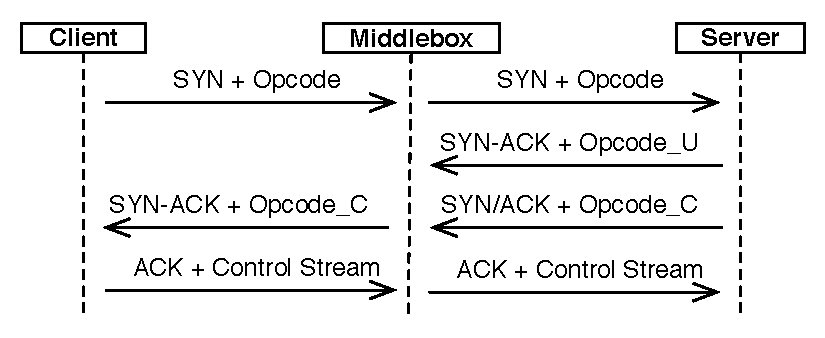
\includegraphics[width=.9\columnwidth]{figs/handshake}
% \vspace{-2mm}
\caption{Example handshake with extension negotiation}
\label{fig:handshake}
\vspace{-4mm}
\end{figure}

An example handshake is shown in Fig.~\ref{fig:handshake}. In this case a client (active opener) sends a SYN packet as show above. The packet traverses a middlebox which does not remove the opcode and reaches the Server (passive opener). The Server replies with SYN-ACK with U\_Opcode which is discarded by the middlebox. It then retransmits SYN-ACK with $Opcode_C$ and Checksum Correction bits, which reaches the Client. The client recovers and verifies the received opcode. Both endpoints are now assumed to understand the meaning of the opcode, therefore the client replies with an ACK with control information acknowledging reception of the $Opcode$ from the Server.

Putting control stream into packet payload suffers from much the same issues as other proposals to extend TCP option space~\cite{Ramaiah:2012wa}. The premise of our work is that middleboxes should not be aware of the new control streams in the first place and therefore not interfere with them.

We witnessed a case of resegmentation where an ACK segment is split to one only acknowledging the received data and another other one with the actual payload. It is not an issue with TLV-encoded control stream in the payload, because it will be delivered to the receiver first. The mechanism of \emph{Checksum Correction} would, however, be compromised for the first segment. If the passive opener receives data during or immediately after the handshake but can not decode that as valid TLV-encoded control information, it treats that as application data and falls back to vanilla TCP.

The focus of our work is to show the possibility of exchanging control information within the packet header. We therefore leave refinement of the full control channel for future work.

\section{Related Work}
\label{sec:related}

Steganography has been used in the past to hide information within network protocols. The main focus has been on covert channels that violate system's security policy and initial sequence numbers~\cite{Rowland:1997vq}, TCP Timestamps~\cite{Giffin:2002wh} and combinations with IP flags~\cite{Murdoch:2005fz}. There are detection techniques for these methods and our main goal is to exchange a small amount of control information rather than a genuine covert channel, asking for a different design.

TCP implements an \emph{urgent mechanism} at its core that allows the sending user to stimulate the receiving user to accept some \emph{urgent data}. The mechanism is often quoted as providing ``out-of-bound'' data delivery even though it is explicitly not designed as a mechanism for sending such data. Furthermore, there are ambiguities regarding the semantics of the urgent pointer, Network Intrusion Detection Systems (NIDS) tend to clear the URG flag and pointer and in general it is recommended against the use of the mechanism~\cite{Gont:2011vi}.

AccECN proposal~\cite{Kuhlewind:2014vd} uses an additional reserved bit, overloads the meaning of already assigned ECN~\cite{Floyd:up} and NS~\cite{Ely:uc} bits and redefines Urgent Pointer as Non-Urgent when URG is not set. The idea is highly related to ours, but reserving the field solely for ECN use prevents other extensions from using. Furthermore, we saw that some networks block packets with such field, making it especially difficult to use for ECN.

Generic control stream for MPTCP~\cite{Bonaventure:wx} can be reused as well. It proposes the mapping control stream into a separate sequence number space and exchange control data over established subflows, only modifying the MPTCP DSS option to differentiate control and data streams. The underlying assumption, however, is that MPTCP is already deployed and that existing deployments will be compatible with the new specification.

%More generally SCTP uses \emph{data chunks} to differentiate between different subflows. Each packet can contain multiple TLV-encoded chunks to separate user data and control information. Despite its challenged deployment in the Internet, SCTP over DTLS is being used as the basis of WebRTC data protocol~\cite{Tuexen:wv} and we suggest that such chunking could be used on top of \emph{noTCP} once control channel has been bootstrapped.

\section{Discussion}

The main points of discussion on \emph{NoTCP} are the same as with all TCP extensions: is it necessary, is it deployable and is it forwards-compatible? We have discussed the first two throughout the paper, but the biggest challenge for forwards-compatibility is NoTCP's overloading of header fields instead of using options.

The exact protocol semantics are subject to further testing and discussions. The main goal of this work is to identify potential methods for exchanging control information by hiding it from existing middleboxes.

In the long term and beyond our example control information exchange we believe that each protocol-relate standards (TCP extensions in this case) should explicitly define which header fields it interferes with and how. Examples include extending sequence numbers and using stronger message integrity checks~\cite{Mazieres:uz}, changing semantics of duplicate ACKs~\cite{Handley:vj,Flach:2013uy} or even simple checksum or window size modifications.

More importantly, we have left open the question of finding a method to hide such information from non-transparent proxies. The easiest, albeit very limited solution is to identify and cache port numbers that allow unmodified traffic. Our goal instead is to study commonly found proxy implementations in detail in order to quickly identify them and encode information within their own operating patterns.

The final goal is to map header field modifications by the various extensions as well as network middleboxes into an algebraic form as we have done in the simple case of checksum. This way we would not only be able to exchange control information across the network reliably, but also identify network path behavior by looking at its performed operations. This way extending a protocol would become a matter of defining a new set of such header algebra rules and simplify the process of design and testing.

\section{Conclusion}

We hope to motivate the research community to explore the full range of possibilities in extending existing protocols. We have developed an Android application to collect data about how network middleboxes interfere with packet header fields that may not currently have a meaning. We encourage more people to install our application to build a comprehensive database of network behavior. The goal of the study is to explore new ways of exchanging control information resilient to major classes of currently deployed middleboxes by using steganographic approaches. 

Finally, we would like to use the results of the study to develop a set of rules for how packet headers are modified by middleboxes as well as standard protocol extensions. If this were true, extending a protocol could become near automatic.

\ifnum\anon=0
\subsection*{Acknowledgments}

\fi


\clearpage
%Only show things we really cite :)
% \nocite{*}
{

\bibliographystyle{abbrv}
\small 
\bibliography{references}
}

%\appendix 
%\input{data}

\end{document}







